%
Als ersten Schritt der digitalen Signalverarbeitung wollen wir uns den \"Ubergang von einem analogen Signal zu einem digitalen n\"aher ansehen.
Intuitiv k\"onnen wir diesen Vorgang in vielen Anwendungen beobachten.
Wir nehmen im Tonstudio mit einem Mikrophon Ton auf und eine Soundkarte wandelt das analoge Signal in einen WAV-Datenstrom um.
In einer Fotokamera, trifft ein Feld von Lichtstrahlen ein und wird von einem \gls{cmos}-Sensor \q{direkt} abgetastet und in Helligkeitswerte pro Farbkanal umgewandelt.
Eine Antenne wandelt ein anliegendes elektro-magnetisches Feld in eine Spannung um, welche nachtr\"aglich von einem \gls{adc} abgetastet und quantisiert wird.

Mathematisch modellieren wir analoge Signale $s_a : D \rightarrow B$ meist mit $D$ und $B$, die auf die reellen Zahlen $\R$ zur\"uckgreifen.
Die Wandlung von analog zu digital transformiert dieses Signal in eine Funktion $s: \Z \rightarrow Q$ um, wobei auch $\Abs{Q} < \infty$ gilt.
Das hei\ss{}t, dass das Signal nach AD-Wandlung nur noch endliche Werte annehmen kann und, dass es nur noch aus eine \emph{Folge} von Werten aus der Menge $Q$ besteht. 
Es wurde also zeit- und wertdiskretisiert.
Wir werden uns zun"achst nur mit der Diskretisierung in Zeit befassen, weil es einfach einfacher ist.
Das hei"st, dass wir uns vorstellen, dass das diskretisierte Signal nur an einer diskreten Menge an Punkten noch Informationen "uber das abgetastete Signal beinhaltet.
Weiterhin sind wir nicht an der physikalischen Umsetzung von \glspl{adc} interessiert, sondern h"ochstens an deren systemtheoretischer Modellierung.

Die zentralen Fragen sind nun:
\begin{itemize}
    \item Wie muss der Vorgang der Abtastung gestaltet sein, dass keine Information verloren geht?
    \item Wie k\"onnen wir die Eigenschaften des analogen Signals in dessen abgetasteter Version wiederfinden?
    \item Welche Operationen k"onnen wir auf digitalen Signalen wie effizient ausf"uhren?
\end{itemize}
%
\subsection{Frequenz von Signalen}
%
\subsubsection{Zeit-Kontinuierliche Harmonische}
%
Meistens werden wir uns in der Vorlesung mit reell- oder komplexwertigen Zeitsignalen befassen, d.h. wir modellieren unsere Signale als $x_a : \R \rightarrow \R$ oder $x_a: \R \rightarrow \C$.
Wobei physikalische Signale nat"urlich nur reellwertig sind, doch manchmal ist die Darstellung als komplexwertige Funktion besser handhabbar, siehe \eqref{complex_baseband}.
Das hei"st, dass die Abtastung im Zeitbereich vonstatten geht, was sofort den Begriff der \emph{Frequenz} auf den Plan ruft, da Frequenz mit Einheit $1/[s]$ eng mit Zeit $[s]$ verkn"upft ist.

Betrachten wir also erst einmal, welchen Einfluss Abtastung von Signalen mit einzelnen Frequenzen hat, am Beispiel von
%
\begin{equation}\label{eq:analog_cosine}
    x_a(t) = A \cos(\Omega t + \theta),
\end{equation}
%
wobei wir hier $A \in \R$ als Amplitude, $\Omega \in \R^+_0$ als Kreisfrequenz $\SI{1}{\radian\per\second}$, $t \in \R$ als Zeit $\SI{1}{\second}$ und die Phase $\theta \in \R$ mit Einheit $\SI{1}{\radian}$ nutzen.
Alternativ k"onnen wir auch zur Frequenz $F \in \R$ $\SI{1}{\per\second} = \SI{1}{\hertz}$ "ubergehen.
Dann erhalten wir
\[
x_a(t) = A \cos(2 \pi F t + \theta).
\]
Diese Funktion ist in \cref{fig:analog_cosine} dargestellt.
Wir sehen, dass die Funktion periodisch ist mit Periode $T_p = 1/F$.

\myemph{Das hei"st, dass $x_a(t + k \cdot T_p)$ f"ur $k \in \Z$ nicht vom Signal $x_a(t)$ zu unterscheiden ist!}

\begin{figure}[t]
    \begin{center}
        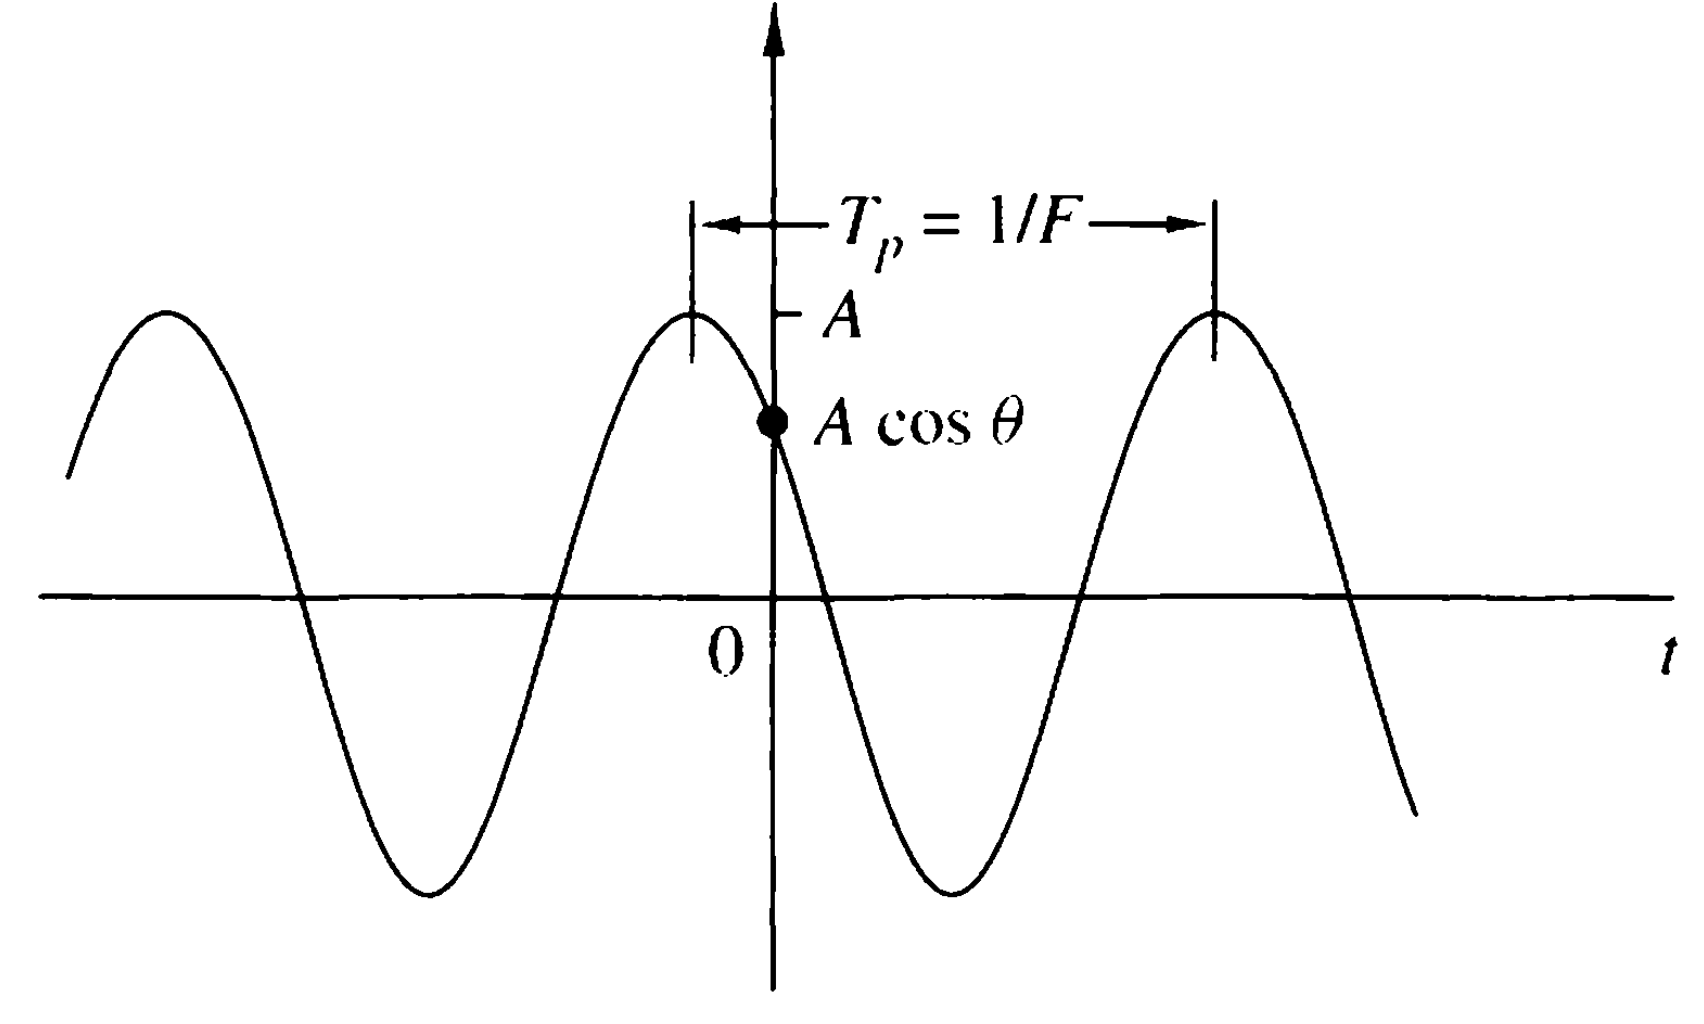
\includegraphics[width=0.48\textwidth]{img/sampling/analog_cosine.png}
        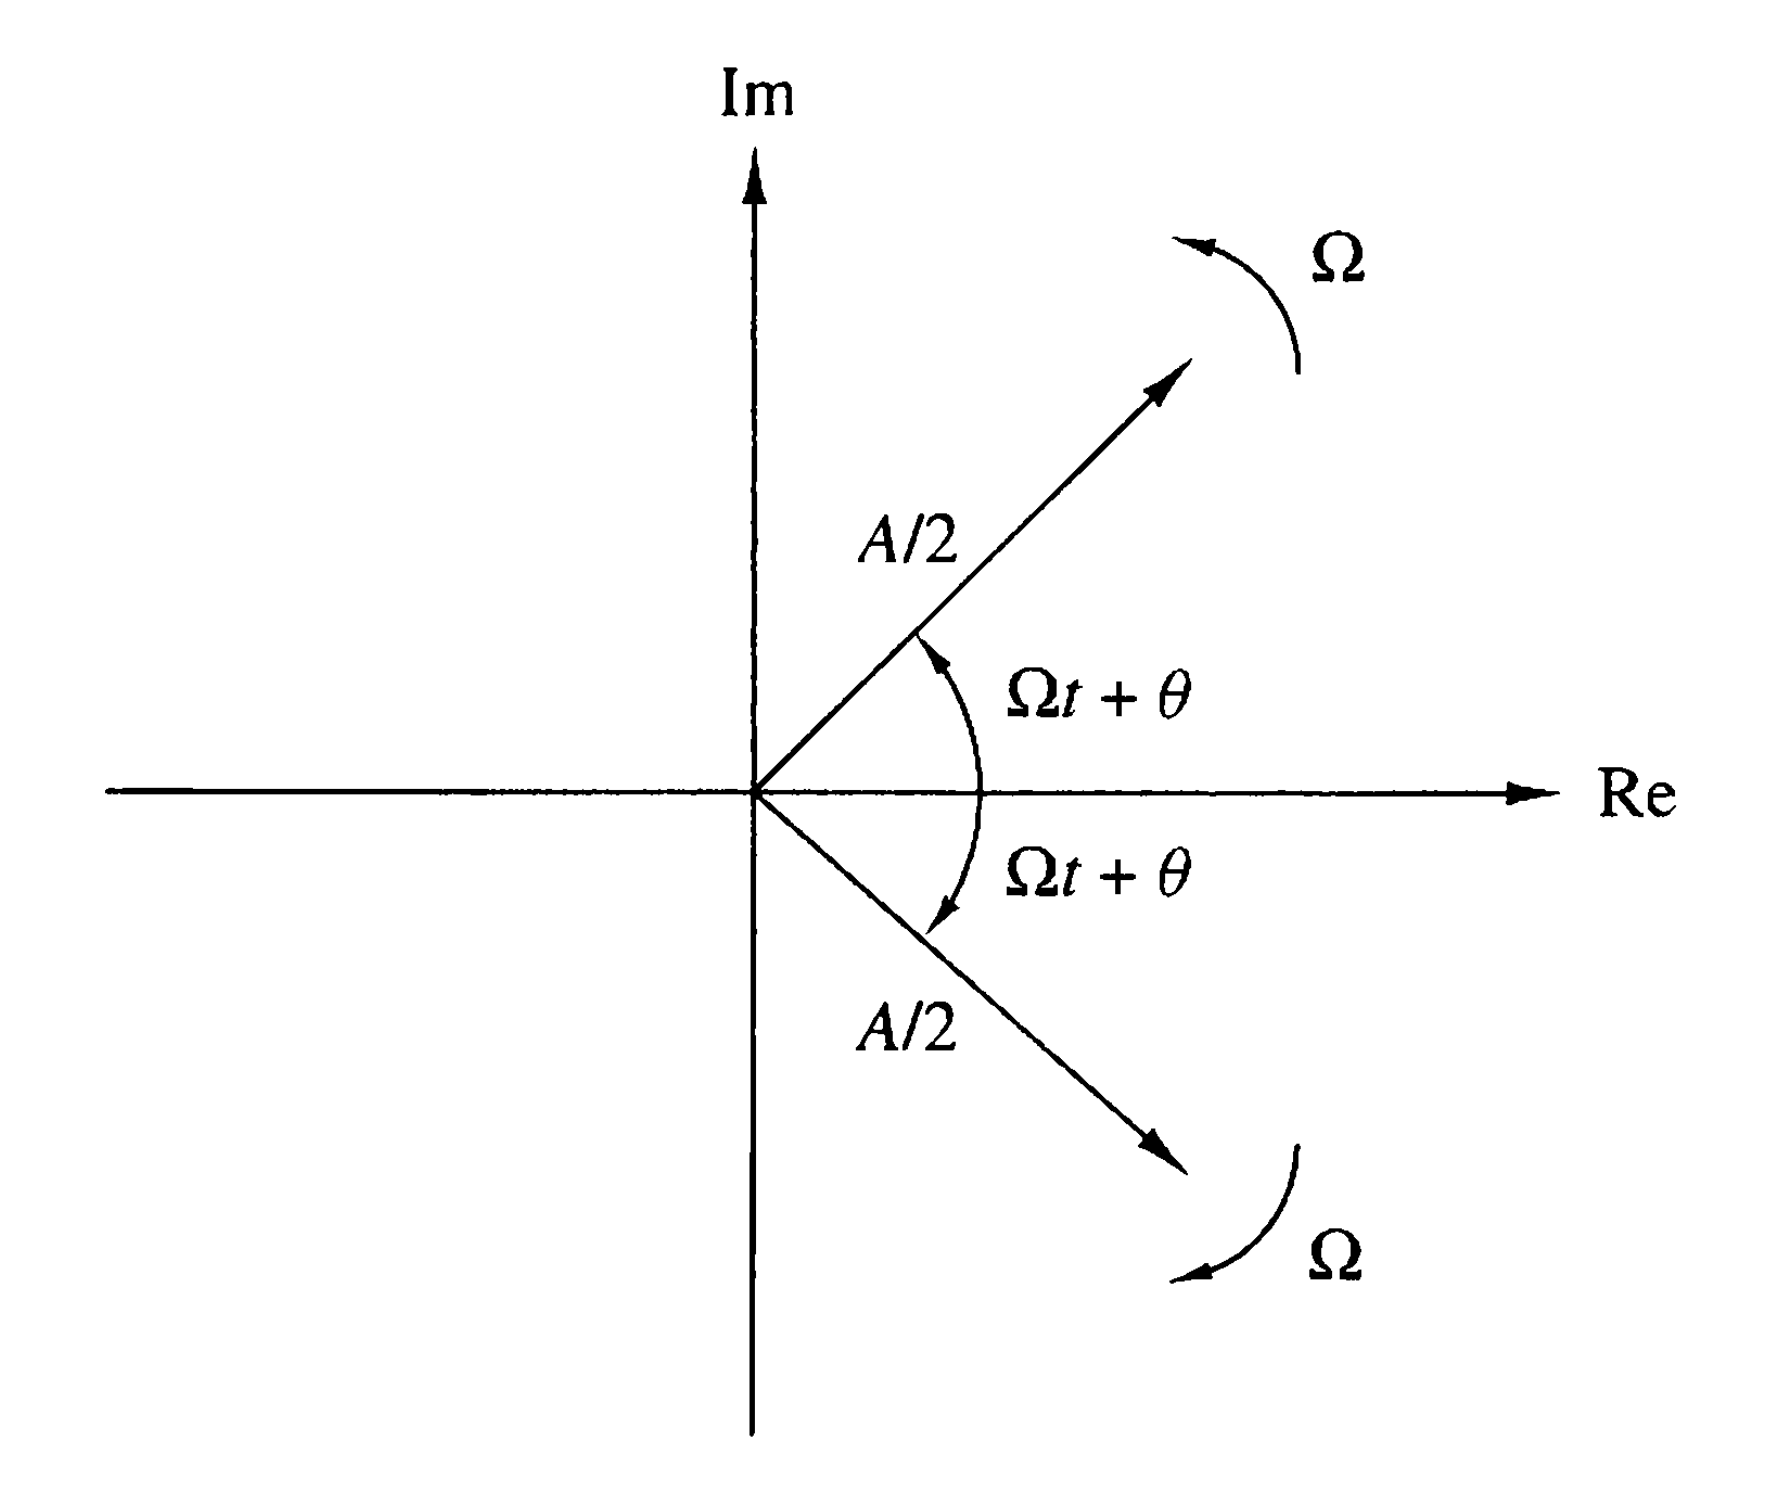
\includegraphics[width=0.48\textwidth]{img/sampling/two_phasors.png}
    \end{center}
    \caption{$x_a(t) = A \cos(2 \pi F t + \theta)$, Quelle: \cite{proakis2013}}\label{fig:analog_cosine}
\end{figure}
%
Es gibt noch eine alternative Darstellung von der obigen Funktion durch die Addition von zwei \emph{Phasoren} als
\[
    x_a(t) 
        = A \cos(2 \pi F t + \theta) 
        = \frac A2 \exp(\jmath (\Omega t + \theta)) 
            + \frac A2 \exp(- \jmath (\Omega t + \theta)).
\]
Da die beiden "uberlagerten Phasoren so interpretiert werden k"onnen als rotierten diese in gegens"atzliche Richtungen, ist es gerechtfertigt der physikalischen Intuition entgegen auch von \q{negativen} Frequenzen zu sprechen.
Wir erlauben also $F \in \R$, womit auch der Spezialfall $T_p = \infty$, also $x_a(t) = A$ abgedeckt ist.
Ein kleines Beispiel findet man in \Cref{py:cont_harms}.
%
\begin{listing}
    \begin{minipage}{0.49\textwidth}
        \inputminted{python3}{code/cont_harms.py}
    \end{minipage}
    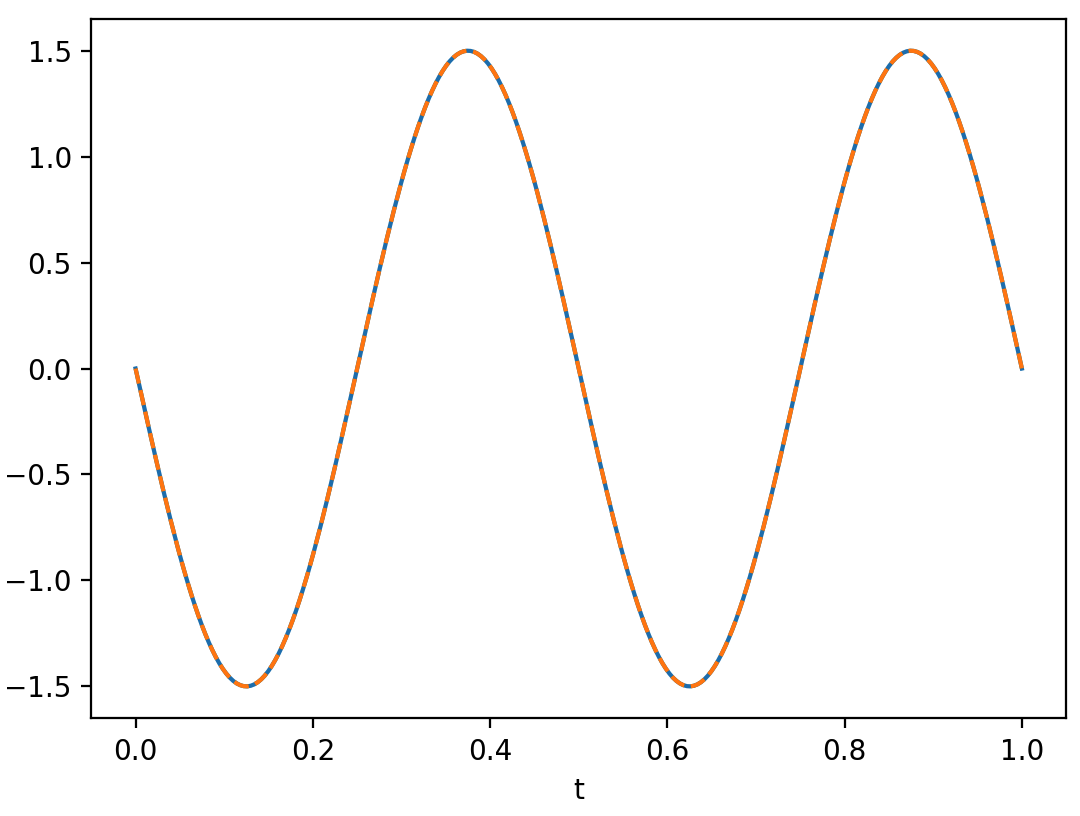
\includegraphics[width=0.49\textwidth]{code/cont_harms.png}
    \caption{Berechnung und Darstellung von \eqref{eq:analog_cosine}}\label{py:cont_harms}
\end{listing}
\FloatBarrier
%
\subsubsection{Zeit-Diskrete Harmonische}
%
Als n"achstes gehen wir zu dem eigentlich interessanten Fall "uber, bei welchem wir von zeitdiskreten harmonischen Signalen sprechen.
Dabei gehen wir vorerst \emph{nicht} davon aus, dass das Signal durch Abtastung eines analogen Signals entstanden ist, sondern betrachten es ganz losgel"ost f"ur sich.
In Analogie zu \eqref{eq:analog_cosine} definieren wir
%
\begin{equation}\label{eq:discrete_cosine}
    x[n] = A \cos(\omega n + \theta) = A \cos(2 \pi f n + \theta).
\end{equation}
%
Wichtig bei diskreten Signalen ist, dass ihre physikalische Interpretierbarkeit nicht direkt gegeben ist, da $n \in \Z$ nur die diskreten Werte \q{nummeriert}, also \emph{einheitenlos} ist.
Deshalb hat $f \in \R$ lediglich als Einheit \q{Zyklen pro Sample}, was man auch daran sieht, dass f"ur $f = 1$ gilt $x[n] = A \cos(2\pi n + \theta) = A \cos(\theta)$.
Es existiert nun ein wichtiger Unterschied zwischen $x[\cdot]$ von \eqref{eq:discrete_cosine} und $x_a(\cdot)$ von \eqref{eq:analog_cosine}.
Das Signal $x[\cdot]$ ist nur periodisch, falls $f$ eine rationale Zahl ist, also $f = p/q$ f"ur $p,q \in \Z$ und $q \neq 0$.

Wieso?

Ein zeitdiskrtes Signal ist periodisch, falls $x[n + N] = x[n]$ f"ur alle $n \in \Z$.
F"ur unser Signal in \eqref{eq:discrete_cosine} hei"st das also, dass
\[
    \cos(2 \pi f n + \theta) 
        = \cos(2 \pi f (n + N) + \theta)
        + \cos(2 \pi f n + 2 \pi f N + \theta)
\]
Da $\cos$ Periode $2\pi k$ f"ur $k \in \Z$ besitzt, muss $2 \pi f N = 2 \pi k$ gelten, also
\[
    f = \frac kN.
\]
Andersherum kann man die kleinste Periode $N$ ermitteln, indem man $f = k/N$ vollst"andig k"urzt, sodass also Z"ahler und Nenner keine gemeinsamen Teiler mehr haben, und man dann den Nenner des resultierenden Bruches als $N$ setzt. 
Ein Beispiel wird in \Cref{py:disc_harms} gezeigt. 
Man kann interessante Ergebnisse erzielen, wenn man diesen Plot f"ur $\omega=0,\pi/8,\pi/4,\pi/2$ und $\omega=\pi$ erzeugt ("Ubung).
%
\begin{listing}
    \begin{minipage}{0.49\textwidth}
        \strut\vspace*{-\baselineskip}\newline
        \inputminted{python3}{code/disc_harms.py}
    \end{minipage}
    \begin{minipage}{0.49\textwidth}
        \strut\vspace*{-\baselineskip}\newline
        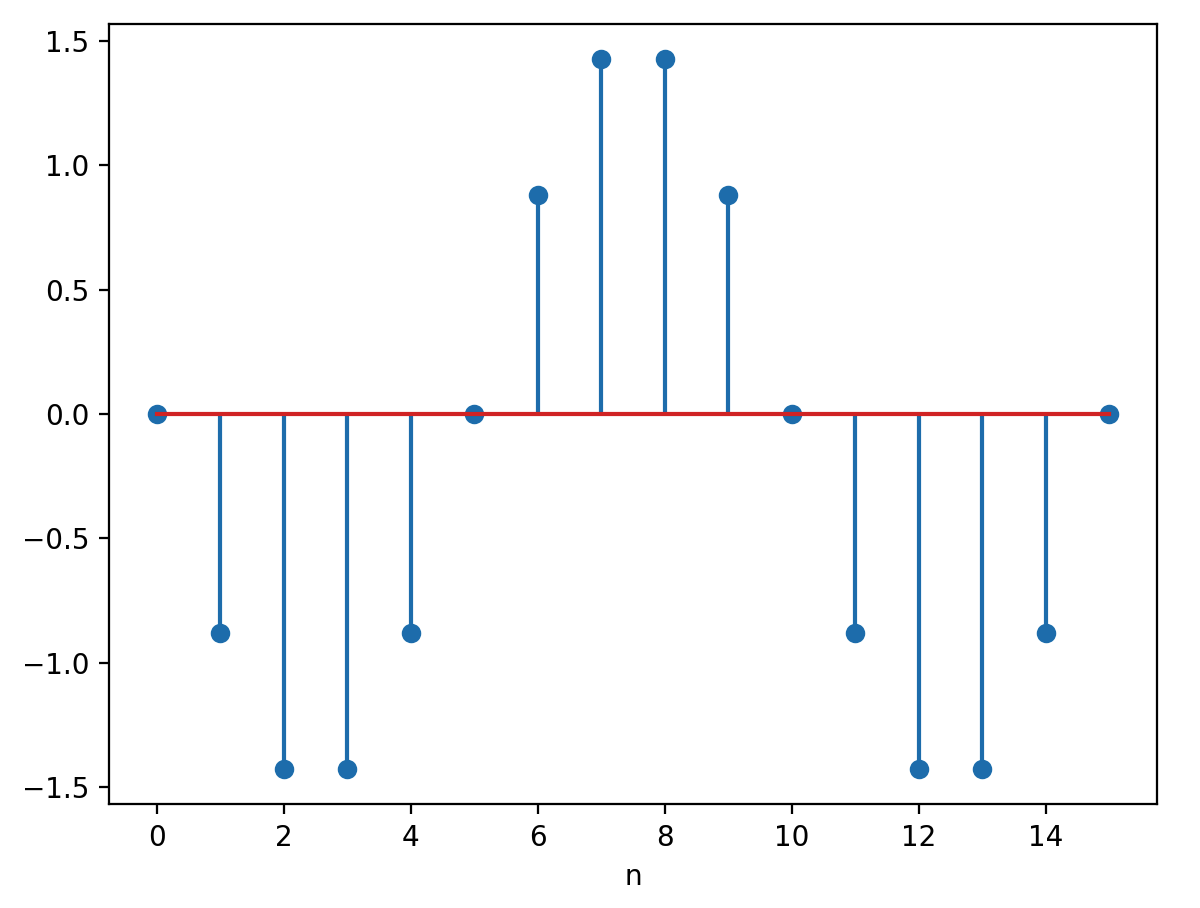
\includegraphics[width=\textwidth]{code/disc_harms.png}
    \end{minipage}
    \caption{Berechnung und Darstellung von \eqref{eq:analog_cosine}}\label{py:disc_harms}
\end{listing}

Die Signale der Form \eqref{eq:discrete_cosine} haben noch eine andere interessante Eigenschaft, die sich wieder aus der $2\pi$-Periodizit"at von $\cos$ ergibt. 
Betrachten wir noch einmal \eqref{eq:discrete_cosine} und wir finden, dass
\[
\cos(\omega n + \theta) = \cos(\omega n + 2\pi n + \theta) = \cos((\omega + 2\pi) n + \theta).
\]
Das hei"st, dass
\[
    x[n] = \cos(\omega n + \theta) = \cos((\omega + 2\pi k) n + \theta) = x_k[n]
\]
f"ur \emph{alle} $k \in \Z$ gilt.
Das hei"st, dass sich $x_k[\cdot]$ nicht von $x[\cdot]$ unterscheiden l"asst.
Man nennt dann jedes der $x_k[\cdot]$ einen \emph{Alias} von $x[\cdot]$.
Man kann deshalb auch sagen, dass f"ur jedes $\omega$ mit $\Abs{\omega} > \pi$ ein zugeh"origes $\omega_a$ mit $\Abs{\omega_a} < \pi$ existiert, sodass
\[
    \cos(\omega n + \theta) = \cos(\omega_a n + \theta)
\]
gilt.
Vergewissern sie sich von dieser Tatsache, indem sie verschiedene Aliase basierend auf \Cref{py:disc_harms} visualisieren ("Ubung).

Stellen wir uns f"ur einen kurzen Moment vor, dass wir wissen, dass wir $x[n]$ durch Abtastung einer Funktion wie in \eqref{eq:analog_cosine} erhalten haben.
Selbst wenn wir wissen, dass nur \emph{eine} Frequenz in diesem Signal vor Abtastung vorhanden war, k"onnen wir \emph{nicht} entscheiden, welche das war.
%
\FloatBarrier
%
\subsection{Zeit-Kontinuierliche Komplexe Harmonische}\label{sec:cont_complex_harm}
%
Wir wollen eine bestimmte Menge an Funktionen betrachten. Wir wollen kontinuierliche komplexe Schwingungen betrachten, welche mit einer Frequenz $F_k$ schwingen, welche ein ganzzahliges Vielfaches einer Frequenz $F_0$ ist.
Das hei"st, wir betrachten dann
\[
F_k = k \cdot F_0 \Text{f"ur} k \in \Z \Text{, was}
x_k(t) = \exp(\jmath 2 \pi F_k t) = \exp(\jmath 2 \pi k F_0 t)
\]
ergibt. 
Jedes der $x_k$ hat Periode $1/F_k = T_k = T_0/k$. 
Das hei"st f"ur wachsendes $\Abs{k}$ werden die Perioden immer um ein Vielfaches k"urzer. 
Umgekehrt haben dann alle $x_k$ gemeinsame Periode, $T_0$, da f"ur jedes $k$ gilt, dass $T_k \cdot k = T_0$.
Wir haben auch kein Problem mit Aliasing zwischen den $x_k$, da bei kontinuierlichen Signalen gilt, dass $x_{k_1} \neq x_{k_2}$, falls $k_1 \neq k_2$.

Wie wir in \Cref{sec:signals_vec} gesehen haben, k"onnen wir beliebige Linearkombination aus Signalen bilden und erhalten wieder ein Signal.
Wir k"onnen also f"ur eine Folge von $c_k \in \C$ die Linearkombination der $x_k$ bilden und erhalten
%
\begin{equation}\label{eq:cont_fourier_series}
    x_a = \Sum{k \in \Z}{}{c_k x_k} : \R \rightarrow \C
    \Text{mit} 
    t \mapsto x_a(t) = \Sum{k \in \Z}{}{c_k x_k(t)}
        = \Sum{k \in \Z}{}{c_k \exp(\jmath 2 \pi k F_0 t)}.
\end{equation}
%
Die erste Schreibweise ist absichtlich ohne das Argument $t$, um zu verdeutlichen, dass Signale \emph{wirklich} als eigenst"andige Signale behandelt werden k"onnen und dass $x_a(t) \in \C$ \q{nur} die Auswertung von $x_a$ an der Stelle $t$ ist, welche \emph{strikt} von dem \emph{Vektor} $x_a$ zu unterscheiden ist.

Nat"urlich ist \eqref{eq:cont_fourier_series} als Fourierreihe von $x_a$ bekannt, und die $c_k$ sind die Fourierkoeffizienten von $x_a$.
Wie in \Cref{sec:signals_vec} k"onnen wir also die $c_k$ durch \eqref{eq:cont_fourier_series} mit $x_a$ \emph{identifizieren}, da uns die $c_k$ eine alternative Darstellung von $x_a$ liefern.
%
\subsection{Zeit-Diskrete Komplexe Harmonische}
%
Analog zu \Cref{sec:cont_complex_harm}, wollen wir uns zeit-diskrete komplexe Schwingungen herleiten, die von einer bestimmten Grundfrequenz definiert werden.
Da wir, im Unterschied zum kontinuierlichen Fall, nicht f"ur alle $f \in \R$ eine periodische Funktion erhalten, w"ahlen wir $f_0 = 1/N$ f"ur ein $N \in \N$. 
Die Intension ist, dass wir so $1/N$ Perioden pro Abtastwert erhalten werden. 
Demzufolge wird die Schwingung mit Frequenz $f_0$ genau Periodenl"ange $N$ haben.
Dann definieren wir die Signale $x_k[\cdot]: \N \rightarrow \C$ als
\[
 x_k[n] = \exp\left(
        \jmath 2 \pi k f_0 n
    \right) \Text{mit} k \in \Z.
\]
Man sieht nun leicht, dass $f_k = k/N$ immer eine rationale Zahl ist und $x_k[\cdot]$ Periodenl"ange $k/N$ hat, falls $k/N \in \Z$.
Au"serdem findet man wieder, dass $x_k[\cdot]$ ein Alias von $x_{k+N}[\cdot]$ sein muss, denn mit $f_0 = 1/N$ ergibt sich
\[
 x_{k+N}[n] = \exp\left(
        \jmath 2 \pi (k + N) f_0 n
    \right)
    = \exp\left(
        \jmath 2 \pi \frac{k + N}{N} n
    \right)
    = \exp\left(
        \jmath 2 \pi \frac{k}{N} n
    \right) 
    \exp\left(
        \jmath 2 \pi \frac NN n
    \right) 
    = x_k[n].
\]
Das hei"st, dass nur $N$ verschiedene $x_k[\cdot]$ existieren.
Normalerweise nimmt man jene $x_k[\cdot]$ f"ur $k = 0, 1, \ldots, N-1$.
Nun k"onnen wir auch wieder, wie in \eqref{eq:cont_fourier_series} eine Linearkombination der $x_k[\cdot]$ bilden.
Man beachte, dass in diesem Fall die Summation nat"urlich \emph{endlich} sein wird, da wir nur $N$ verschiedene $x_k[\cdot]$ zur Verf"ugung haben.
Wir bilden also
\[
    x[\cdot] = \Sum{k = 0}{N-1}{c_k x_k[\cdot]}
\]
und erhalten so ein Signal mit Werten
\begin{equation}\label{eq:disc_fourier_series}
    x[n] 
        = \Sum{k = 0}{N-1}{c_k x_k[n]} 
        = \Sum{k = 0}{N-1}{
            c_k \exp\left(
                \jmath 2 \pi \frac{k}{N} n
            \right) 
        },
\end{equation}
was die Fourierreihe eines diskreten und periodischen Signals darstellt, wobei in diesem Fall der Vektor $\bm c = [c_k]_{k=0}^{N-1} \in \C^N$ eine alternative Repr"asentation des Signals ist.

Das Signal $x[\cdot]$ selbst ist periodisch mit Periodenl"ange $N$, d.h. das Signal ist durch die Werte $\bm x = [x[n]]_{n=0}^{N-1} \in \C^N$ \emph{vollst"andig} definiert. Das hei"st wir k\"onnen das Signal $x[\cdot]$ mit dem \emph{endlich-dimensionalen} Vektor $\bm x \in \C^N$ identifizieren.
Da genauso jedes der $x_k[\cdot]$ auch Periodenl"ange $N$ hat, erhalten wir auf die gleiche Weise Vektoren $\bm x_k \in \C^N$.
Mit diesen endlich-dimensionalen Vektoren sind wir nun in der Lage die Fourierreihe in \eqref{eq:disc_fourier_series} mit \q{normalen} Vektoren durch
%
\begin{equation}\label{eq:disc_fourier_lincomb}
    \bm x = c_1 \bm x_1 + c_2 \bm x_2 + \ldots + c_{N-1} \bm x_{N-1}
\end{equation}
%
auszudr"ucken.
Wir sehen also \emph{direkt}, dass Signale wirklich wie Vektoren behandelt werden k"onnen.

\Cref{eq:disc_fourier_series} kann auch als Abbildung $M : \C^N \rightarrow \C^N$ interpretiert werden, da wir in die rechte Seite von \eqref{eq:disc_fourier_series} einfach ein $\bm c \in \C^N$ stecken k"onnen und wir erhalten das entsprechende $\bm x = M(\bm c)$.
Noch weiter ist die Abbildung $M$ sogar linear, da 
\[
    M(\bm c^1 + \bm c^2)
        =  \Sum{k = 0}{N-1}{
            (c^1_k + c^2_k) \exp\left(
                \jmath 2 \pi \frac{k}{N} n
            \right) 
        }
        =  \Sum{k = 0}{N-1}{
            c^1_k \bm x_k
        }
        + \Sum{k = 0}{N-1}{
            c^2_k \bm x_k 
        }
        = M(\bm c^1) + M(\bm c^2).
\]
Das hei"st, dass es auch eine \emph{Matrix} $\bm M \in \C^{N \times N}$ geben muss, welche uns einfach $\bm c$ in $\bm x$ umtransformiert, indem wir $\bm x = \bm M \cdot \bm c$ als Matrix-Vektor-Produkt berechnen.
Wenn wir \eqref{eq:disc_fourier_lincomb} genau betrachten sehen wir, dass wir die Matrix $\bm M$ bilden k"onnen, indem wir deren $k$-te Spalte $\bm M_{\cdot, k}$ gleich $\bm x_k$ setzen.
Wenn wir noch sicher sein k"onnten, dass $\bm M$ invertierbar ist, k"onnten wir sogar aus $\bm x$ via $\bm c = \bm M^{-1} \cdot \bm x$ die Fourierkoeffizienten $\bm c$ direkt aus einem gegebenen $N$-periodischen Signal $x[\cdot]$ bestimmen.
%
%
\subsection{Finally: Abtastung von Signalen}
%
Es gibt viele M"oglichkeiten ein analoges Signal zu digitalisieren.
Wir beschr"anken uns auf Abtastung, welche ein analoges Signal auf eine regelm"a"sige Art und Weise \emph{direkt} auswertet.
Diese Art wird manchmal auch \q{Nyquist-Sampling} genannt, weil die theoretische Grundlage f"ur \q{erfolgreiches} Sampling durch das Nyquist-Theorem gelegt ist.
Wir stellen uns Abtastung so vor, dass wir das Signal $x_a: \R \rightarrow \R$ direkt an gewissen Stellen beobachten k"onnen.
Wir k"onnen uns eine Art Sampling-Operator $\mathcal{S}$ vorstellen, der ein analoges Signal $x_a$ in eine abgetastete Version $x_a \mapsto \mathcal{S}(x_a)[\cdot] = x[\cdot]$ transformiert.
Durch die regelm"a"sige Abtastung in Zeitabst"anden $T > 0$ von $x_a$ erhalten wir also
\[
    x[n] = \mathcal{S}(x_a)[n] = x_a(n T) \Text{mit} n \in \Z.
\]
Wir nennen $F_s = T^{-1}$ die Sampling-Frequenz, oder die Abtastrate.

Da wir uns $x[\cdot]$ so vorstellen, dass es \q{einfach} eine Folge von reellen Zahlen ist, m"ussen wir bei der Interpretation von $x[\cdot]$ auch immer gleichzeitig im Hinterkopf behalten, dass der Wert $x[n]$ dem Wert $x_a(n T) = x_a(n/F_s)$ entspricht.
Das bedeutet, dass $t$ (als Argument von $x_a$) und $n$ (als Argument von $x[\cdot]$) durch
\[
t = n T = n/F_s
\]
miteinander in Verbindung stehen. 
Man sieht auch nun eindrucksvoll, dass dadurch $n = t \cdot F_s$ einheitenlos geworden ist, bzw.~sein muss.

